\chapter{Despliegue y Puesta en Producción}
\label{cap:despliegue}

\section{Introducción}
\label{sec:intro_despliegue}

Este capítulo describe el proceso de transición del sistema \textit{CORE-MP} desde el entorno de experimentación —basado en \textit{notebooks} de Jupyter— hasta un despliegue real y reproducible en producción. Esta fase, conocida en la industria como \textit{MLOps} (\textit{Machine Learning Operations}), constituye uno de los pasos más críticos en el ciclo de vida de cualquier modelo de aprendizaje automático: sin ella, los modelos entrenados permanecen confinados en el entorno del científico de datos y no generan valor real para el usuario final.

La transición a producción implica resolver una serie de retos técnicos que van más allá del modelado:

\begin{itemize}
    \item \textbf{Reproducibilidad:} garantizar que el entorno de ejecución del modelo es idéntico en cualquier máquina, independientemente del sistema operativo o las dependencias instaladas localmente.
    \item \textbf{Separación de responsabilidades:} distinguir claramente entre el proceso de entrenamiento (que ocurre de forma periódica o puntual) y el servicio de inferencia (que debe estar disponible de forma continua).
    \item \textbf{Consistencia del preprocesado:} asegurar que las transformaciones aplicadas a los datos en tiempo de entrenamiento se replican de forma exacta en tiempo de inferencia, evitando el denominado \textit{training-serving skew}.
    \item \textbf{Observabilidad:} instrumentar el sistema para medir su rendimiento en producción y detectar degradaciones del modelo a lo largo del tiempo.
\end{itemize}

La solución adoptada en este proyecto se basa en tres pilares tecnológicos: \textbf{FastAPI} como framework para la construcción de la API REST, \textbf{Docker} como mecanismo de containerización y \textbf{una arquitectura modular en Python} que separa limpiamente cada responsabilidad del sistema.

\section{Arquitectura del Sistema}
\label{sec:arquitectura_despliegue}

\subsection{Visión General}
\label{subsec:vision_general}

El sistema de producción se compone de \textbf{dos contenedores Docker independientes} con ciclos de vida distintos:

\begin{itemize}
    \item \textbf{Contenedor de entrenamiento (\texttt{train}):} ejecuta el pipeline completo de ingesta, ingeniería de características y entrenamiento de modelos. Se trata de un contenedor de \textit{ejecución única}: arranca, entrena, serializa los modelos en disco y termina. No es un servicio persistente.
    \item \textbf{Contenedor de inferencia (\texttt{api}):} carga los modelos serializados desde el volumen compartido y expone una API REST que permanece activa indefinidamente, respondiendo peticiones de predicción en tiempo real.
\end{itemize}

La comunicación entre ambos contenedores se realiza exclusivamente a través de un \textbf{volumen Docker compartido} (\texttt{models\_output/}), en el que el contenedor de entrenamiento escribe los artefactos del modelo y el contenedor de inferencia los lee. Este mecanismo de desacoplamiento garantiza que ningún contenedor necesita conocer los detalles internos del otro.

\begin{figure}[H]
\centering
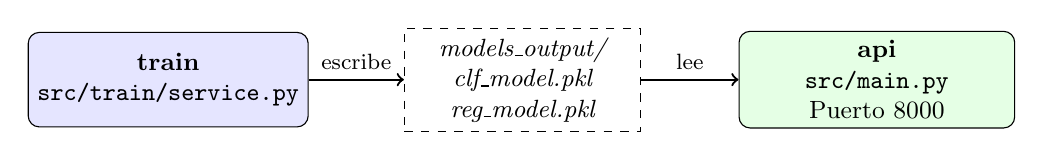
\begin{tikzpicture}[
    box/.style={rectangle, draw, rounded corners, minimum width=3.5cm, minimum height=1.2cm, align=center, font=\small},
    arrow/.style={->, thick},
    vol/.style={rectangle, draw, dashed, minimum width=3cm, minimum height=1cm, align=center, font=\small\itshape}
]
    \node[box, fill=blue!10] (train) at (0,0) {\textbf{train}\\\texttt{src/train/service.py}};
    \node[vol] (vol) at (4.5,0) {models\_output/\\clf\_model.pkl\\reg\_model.pkl};
    \node[box, fill=green!10] (api) at (9,0) {\textbf{api}\\\texttt{src/main.py}\\Puerto 8000};
    \draw[arrow] (train) -- node[above]{\footnotesize escribe} (vol);
    \draw[arrow] (vol) -- node[above]{\footnotesize lee} (api);
\end{tikzpicture}
\caption{Arquitectura de dos contenedores del sistema CORE-MP. El volumen compartido actúa como contrato entre el pipeline de entrenamiento y el servicio de inferencia.}
\label{fig:arquitectura_docker}
\end{figure}

\subsection{Justificación del Diseño}
\label{subsec:justificacion_diseno}

La decisión de separar entrenamiento e inferencia en contenedores independientes responde a principios fundamentales de arquitecturas de sistemas en producción:

\begin{enumerate}
    \item \textbf{Independencia de ciclos de vida:} el reentrenamiento del modelo no requiere interrumpir el servicio de inferencia. Basta con ejecutar el contenedor de entrenamiento, sustituir los artefactos en el volumen y reiniciar la API.
    \item \textbf{Menor superficie de ataque:} el contenedor de inferencia no incluye las dependencias de entrenamiento (e.g., \texttt{scikit-learn} completo con sus utilidades de selección de modelos), lo que reduce el tamaño de la imagen y el número de dependencias externas.
    \item \textbf{Escalabilidad diferenciada:} en un entorno de producción real, el servicio de inferencia puede escalarse horizontalmente (múltiples réplicas) mientras el entrenamiento permanece como proceso \textit{batch} único.
\end{enumerate}

\section{Pipeline de Ingeniería de Características en Producción}
\label{sec:features_produccion}

\subsection{El Principio Stateless / Stateful}
\label{subsec:stateless_stateful}

Una de las decisiones de diseño más críticas en la transición a producción es la gestión del preprocesado de datos. En el sistema implementado, todas las transformaciones de ingeniería de características se centralizan en el módulo \texttt{src/features/service.py} y se clasifican según su naturaleza:

\begin{itemize}
    \item \textbf{Transformaciones \textit{stateless} (sin estado):} operaciones que se calculan directamente a partir de los datos de entrada, sin requerir parámetros ajustados previamente. En este proyecto, la totalidad de las 23 características derivadas (diferencias absolutas entre perfiles, indicadores binarios de coincidencia, distancias de personalidad y el \texttt{overall\_match\_score}) son de este tipo. La función \texttt{create\_pair\_features()} encapsula estas transformaciones y se invoca de forma idéntica tanto durante el entrenamiento como durante la inferencia.

    \item \textbf{Transformaciones \textit{stateful} (con estado):} operaciones que requieren parámetros calculados sobre el conjunto de entrenamiento y que deben serializarse para ser reutilizados en inferencia, como escaladores (\texttt{StandardScaler}) o límites de \textit{outliers}. En este proyecto, el \texttt{StandardScaler} se integra dentro del \textit{pipeline} de \texttt{scikit-learn} del modelo de clasificación y se serializa conjuntamente con él, garantizando que los parámetros de escalado aprendidos en entrenamiento se aplican de forma idéntica en inferencia.
\end{itemize}

Esta separación es la que previene el \textit{training-serving skew}: el error más común y costoso en sistemas de \textit{Machine Learning} en producción, que se produce cuando las transformaciones aplicadas a los datos en tiempo de inferencia difieren —aunque sea sutilmente— de las aplicadas durante el entrenamiento.

\section{Implementación de la API REST}
\label{sec:api_rest}

\subsection{Framework y Tecnología}
\label{subsec:framework}

La API de inferencia se implementa con \textbf{FastAPI}~\cite{fastapi}, un framework moderno de Python para la construcción de APIs REST con alto rendimiento, validación automática de tipos mediante \textbf{Pydantic} y generación automática de documentación interactiva en formato OpenAPI (accesible en \texttt{/docs}).

La elección de FastAPI frente a alternativas como Flask o Django REST Framework se justifica por:

\begin{itemize}
    \item \textbf{Validación declarativa:} los modelos Pydantic definen el contrato de entrada y salida de la API de forma explícita, rechazando automáticamente peticiones malformadas con mensajes de error descriptivos.
    \item \textbf{Rendimiento:} FastAPI está construido sobre \texttt{Starlette} y \texttt{uvicorn}, alcanzando rendimientos comparables a frameworks asíncronos de otros lenguajes.
    \item \textbf{Documentación automática:} la especificación OpenAPI se genera sin código adicional, facilitando la integración con sistemas externos.
\end{itemize}

\subsection{Gestión del Ciclo de Vida}
\label{subsec:lifespan}

Un aspecto crítico de la API es la carga de los modelos. Se adopta el patrón \textbf{\textit{fail-fast}}: los modelos se cargan \textbf{una única vez} en el arranque del servidor, mediante el gestor de ciclo de vida (\textit{lifespan}) de FastAPI, y se almacenan en \texttt{app.state}. Si alguno de los ficheros \texttt{.pkl} no existe en el momento del arranque, el servidor falla inmediatamente con un error claro, evitando que la API quede activa sin modelos disponibles. Este comportamiento es preferible a detectar el fallo en el momento de la primera petición.

La inyección de dependencias (\texttt{Depends}) permite que los \textit{endpoints} accedan al predictor y al \textit{tracker} de métricas sin acoplarse a variables globales, mejorando la testabilidad y la claridad del código.

\subsection{Endpoints Disponibles}
\label{subsec:endpoints}

La API expone tres \textit{endpoints}, agrupados en dos dominios funcionales:

\begin{table}[H]
\centering
\footnotesize
\begin{tabular}{llp{8.5cm}}
\hline
\textbf{Método} & \textbf{Ruta} & \textbf{Descripción} \\ \hline
\texttt{POST} & \texttt{/predict}  & Recibe los perfiles de dos personas y devuelve la predicción de compatibilidad y longevidad estimada. \\
\texttt{GET}  & \texttt{/health}   & Comprueba que el servicio está activo y los modelos están cargados. \\
\texttt{GET}  & \texttt{/metrics}  & Devuelve métricas acumuladas de latencia: número de peticiones, latencia total y latencia media. \\ \hline
\end{tabular}
\caption{Endpoints de la API REST del sistema CORE-MP.}
\label{tab:endpoints_api}
\end{table}

\subsection{Esquema de Entrada y Salida}
\label{subsec:esquema_api}

El \textit{endpoint} principal \texttt{POST /predict} acepta un objeto JSON con los perfiles de las dos personas (\texttt{person\_a} y \texttt{person\_b}), cada uno con los 13 atributos originales del \textit{dataset}. La respuesta incluye:

\begin{itemize}
    \item \textbf{\texttt{compatible}:} clasificación binaria (\textit{true}/\textit{false}), derivada del umbral de probabilidad $p \geq 0{,}5$.
    \item \textbf{\texttt{compatibility\_probability}:} probabilidad estimada por la Regresión Logística, en el intervalo $[0, 1]$.
    \item \textbf{\texttt{estimated\_longevity\_months}:} duración estimada de la relación en meses, obtenida invirtiendo la transformación logarítmica aplicada durante el entrenamiento ($\hat{y} = e^{\hat{y}_{\log}} - 1$).
    \item \textbf{\texttt{overall\_match\_score}:} puntuación global de compatibilidad calculada durante el \textit{feature engineering}, con valor en $[0, 1]$.
    \item \textbf{\texttt{latency\_ms}:} tiempo de procesamiento de la petición en milisegundos.
\end{itemize}

\section{Containerización con Docker}
\label{sec:docker}

\subsection{Imágenes Docker}
\label{subsec:imagenes_docker}

Cada uno de los dos contenedores se construye a partir de una imagen Docker independiente, definida en su propio \textit{Dockerfile}:

\begin{itemize}
    \item \textbf{\texttt{Dockerfile.train}:} utiliza \texttt{python:3.12-slim} como imagen base. Instala las dependencias del fichero \texttt{requirements.txt} y ejecuta el módulo \texttt{src.train.service} al arrancar, lo que desencadena el pipeline completo de entrenamiento.
    \item \textbf{\texttt{Dockerfile.api}:} utiliza la misma imagen base. Arranca el servidor \texttt{uvicorn} apuntando al módulo \texttt{src.main:app}, exponiendo el puerto 8000.
\end{itemize}

En ambos casos, las dependencias se instalan como primera capa de la imagen, aprovechando el sistema de caché de Docker: si el fichero \texttt{requirements.txt} no cambia entre construcciones, esta capa se reutiliza, reduciendo el tiempo de \textit{build} significativamente.

\subsection{Orquestación con Docker Compose}
\label{subsec:docker_compose}

El fichero \texttt{docker-compose.yml} orquesta ambos servicios y gestiona la comunicación a través de volúmenes:

\begin{itemize}
    \item El servicio \texttt{train} monta el directorio \texttt{./data/raw} (solo lectura) para acceder al \textit{dataset}, y el directorio \texttt{./models\_output} (lectura y escritura) para depositar los modelos entrenados.
    \item El servicio \texttt{api} monta el directorio \texttt{./models\_output} (solo lectura) para cargar los modelos, y expone el puerto \texttt{8000:8000} al \textit{host}.
    \item Las rutas de los modelos y del \textit{dataset} se inyectan a través de variables de entorno, definidas centralmente en \texttt{src/config.py}, lo que permite sobreescribir cualquier parámetro sin modificar el código fuente.
\end{itemize}

El flujo de ejecución recomendado es secuencial: primero se lanza el contenedor de entrenamiento hasta su terminación y, a continuación, se arranca el servicio de API:

\begin{enumerate}
    \item \texttt{docker compose run --rm train}
    \item \texttt{docker compose up api}
\end{enumerate}

\section{Estructura Modular del Código}
\label{sec:estructura_modular}

\subsection{Organización por Dominio Funcional}
\label{subsec:organizacion_modular}

El código fuente del sistema sigue una arquitectura orientada a dominios funcionales, inspirada en las convenciones de proyectos FastAPI de nivel empresarial.

Esta estructura garantiza que cada componente tenga una única responsabilidad (\textit{Single Responsibility Principle}) y que los cambios en un dominio no afecten a los demás. Por ejemplo, una modificación en el esquema de la respuesta de la API solo requiere editar \texttt{src/infer/schemas.py}, sin alterar la lógica de predicción ni la de monitoreo.

\section{Estrategia de Monitoreo}
\label{sec:monitoreo}

\subsection{Métricas de Latencia}
\label{subsec:metricas_latencia}

El monitoreo de un sistema de \textit{Machine Learning} en producción es una condición necesaria para detectar degradaciones del modelo (\textit{model drift}) o problemas de rendimiento de la infraestructura. En el sistema implementado, cada petición al \textit{endpoint} \texttt{/predict} registra su tiempo de procesamiento, acumulado en el objeto \texttt{MetricsTracker} almacenado en \texttt{app.state}.

La \textbf{latencia media} del sistema se calcula como:

\begin{equation}
    \bar{L} = \frac{\displaystyle\sum_{i=1}^{N} \left( t_{\text{respuesta},i} - t_{\text{solicitud},i} \right)}{N}
    \label{eq:latencia_media}
\end{equation}

donde $t_{\text{solicitud},i}$ es el instante en que se recibe la $i$-ésima petición, $t_{\text{respuesta},i}$ es el instante en que se envía la respuesta correspondiente, y $N$ es el número total de peticiones procesadas.

Esta métrica es accesible en tiempo real mediante \texttt{GET /metrics}, que devuelve el número total de peticiones, la latencia acumulada y la latencia media, todo ello calculado de forma \textbf{\textit{thread-safe}} mediante un \texttt{threading.Lock}, garantizando la consistencia de los contadores bajo carga concurrente.

\subsection{Comprobación de Estado (\textit{Health Check})}
\label{subsec:health_check}

El \textit{endpoint} \texttt{GET /health} devuelve el estado operativo del servicio, indicando si los modelos están cargados correctamente y la versión de la API. Este \textit{endpoint} puede ser consumido por herramientas de orquestación (como Kubernetes o Docker Swarm) para determinar si el contenedor está listo para recibir tráfico (\textit{readiness probe}).

\section{Conclusiones}
\label{sec:conclusiones_despliegue}

El proceso de despliegue del sistema \textit{CORE-MP} ha permitido materializar los modelos entrenados en el Capítulo~\ref{cap:modelado} en un servicio real, reproducible y observable. Las principales conclusiones son:

\begin{enumerate}
    \item \textbf{La separación de entrenamiento e inferencia} en contenedores independientes es el principio más importante del despliegue. Permite actualizar el modelo sin interrumpir el servicio y escalar ambos componentes de forma independiente según sus necesidades.

    \item \textbf{El patrón \textit{stateless}} en el \textit{feature engineering} garantiza la consistencia entre entrenamiento e inferencia. Al centralizar las transformaciones en \texttt{src/features/service.py} y aplicarlas de forma idéntica en ambos contextos, se elimina por diseño la posibilidad de \textit{training-serving skew}.

    \item \textbf{La arquitectura modular} organizada por dominio funcional (\texttt{features}, \texttt{train}, \texttt{infer}, \texttt{monitor}) mejora la mantenibilidad y permite que equipos distintos trabajen sobre componentes independientes sin interferencias.

    \item \textbf{El patrón \textit{fail-fast}} en la carga de modelos garantiza que el sistema no queda activo en un estado inconsistente: si los artefactos del modelo no están disponibles en el arranque, el servidor falla inmediatamente con un error claro y descriptivo.

    \item \textbf{El monitoreo de latencia} incorporado desde el primer día, con métricas accesibles vía API, sienta las bases para una evolución hacia sistemas de detección de \textit{drift} más sofisticados, que podrían alertar cuando la distribución de los datos de entrada en producción se aleja de la distribución de entrenamiento.
\end{enumerate}

Como líneas de trabajo futuro en el ámbito del despliegue, se plantea la integración de \textbf{MLflow} para el registro y versionado de experimentos, el uso de \textbf{MinIO} como almacenamiento de artefactos compatible con S3, y la orquestación del sistema sobre \textbf{Kubernetes} para entornos de producción con alta disponibilidad y escalado automático.
